\chapter{Preliminaries}

\section{Graph Matching}

\subsection{Bipartite Matching}

A graph is called \emph{bipartite} if its vertex set can be 
partitioned into two disjoint set $U$ and $V$ such that every edge
connects a vertex in $U$ with a vertex in $V$. Such a graph is often 
written as $G = (U, V, E)$ where $U$ and $V$ are two disjoint vertex set
and $E$ is the edge set.

A \emph{matching} in a graph $G = (U, V, E)$ is a set of edges $M$ such
that no two edges shared a common vertex. And a matching $M$ is called 
\emph{maximal} if for every edge $e \in E \setminus M$ it satisfies that
$e$ shares some common vertices with some edges from $E$.
Normally we are interested in the \emph{maximum} matching, i.e.\ a matching
containing the largest possible number of edges. And the size of the
maximum matching is called the \emph{matching number} of this graph.
Figure~\ref{maximummatching} shows an example of a maximum matching in
a bipartite graph. Note that the problem of finding a maximum matching 
can be solved in polynomial time by \emph{Hungarian method}.

People show their great interests in finding the maximum matching since
there are deep connections between the matching number and many other
interesting properties in a given graph. 
For example, the \emph{K\"{o}nig's theorem} proved by D\'{e}nes K\H{o}nig
in 1931 states that, in bipartite graph, it is equivalent to find 
a maximum matching that to find a minimum set cover. Independently in
the same year by Jen\H{o} Egerv\'{a}ry the same result was shown in the
more general case of weighted bipartite graphs. Thus a lot of problems
was shown to be NP-hard in general graphs have a polynomial time
algorithm in bipartite graphs (e.g.\ minimum set cover).

\begin{figure}\centering
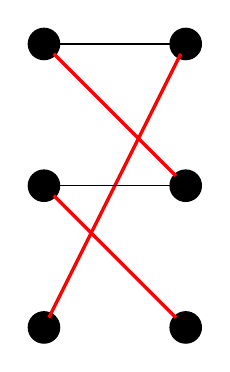
\begin{tikzpicture}[node distance=1.8cm]
    \node   (1)     {};
    \node   (2) [right of = 1]    {};
    \node   (3) [above of = 1]    {};
    \node   (4) [right of = 3]    {};
    \node   (5) [above of = 3]    {};
    \node   (6) [right of = 5]    {};

    \draw[fill=black]   (1) circle (0.2cm);
    \draw[fill=black]   (2) circle (0.2cm);
    \draw[fill=black]   (3) circle (0.2cm);
    \draw[fill=black]   (4) circle (0.2cm);
    \draw[fill=black]   (5) circle (0.2cm);
    \draw[fill=black]   (6) circle (0.2cm);

    \draw[very thick, red]   (1) --  (6);
    \draw[very thick, red]   (3) --  (2);
    \draw[very thick, red]   (5) --  (4);
    \draw   (5) --  (6);
    \draw   (3) --  (4);
\end{tikzpicture}
\label{maximummatching}
\caption{The red edges forms a maximum matching in graph}
\end{figure}

\subsection{Weighted Bipartite Matching}

To generalize the maximum matching problem we could assign weights to those
edges. And the goal is then changed to find a matching with the 
largest/smallest possible weight. This gives us the \emph{maximum/minimum
weighted bipartite matching problem}.

Formally speaking, given a weighted complete bipartite graph
$G = (U, V, w)$ where $U$ and $V$ are two disjoint vertex sets and the edge
set $E = U \times V$. $w$ is the weight function maps every edge in $E$ 
to its own weight in $\mathbb{R}$. We have to find a matching $M$ such that
its weight $w(M) \triangleq \sum_{e \in M} w(e)$ is maximized/minimized.

This maximum weighted bipartite matching problem characterized a lot of
problems in our daily lives. For example we are selling some items 
(e.g.\ potato, orange and banana) and the customers 
(e.g.\ alice, bob and celine) provides their prices on each of these items.
Every customer wants only one item and a item could only be sold to one of
the customers. The problem is how are we going to sell these items so that
we can earn the most money. Figure~\ref{matchingexample} shows an example
of such a problem, and it is clear that we should sell potato to alice, 
orange to celine and banana to bob so that we can earn $5 + 6 + 7 = 18$ in
total.

\begin{figure}
\begin{center}
\begin{tabular}{| c | c | c | c |}
    \hline
        & potato & orange & banana \\
    \hline
        alice & {\bf \color{red} 5} & 3 & 1 \\
    \hline
        bob & 2 & 4 & {\bf \color{red} 7} \\
    \hline
        celine & 3 & {\bf \color{red} 6} & 4 \\
    \hline
\end{tabular}
\end{center}
\label{matchingexample}
\caption{An example of maximum weighted bipartite matching}
\end{figure}

To solve the maximum/minimum weighted bipartite matching problem, a 
polynomial-time algorithm was proposed by Harold~\cite{kuhn1955hungarian}, 
who gives the name ``\emph{Hungarian method}" as this algorithm was 
largely based on the works done by two Hungarian mathematicians 
D\'{e}nes K\H{o}nig and Jen\H{o} Egerv\'{a}ry.

\section{Online Algorithms}

But most of time in our real lives, our information about the graph is
usually incomplete. And we have to make our decisions before the whole
graph is shown to us.

For example in figure~\ref{matching example}, when Alice comes and wants
to buy one item, we can not let her wait until Bob and Celine provide their
prices. We have to make our decision right now on which one to sell before
Alice gets angry. This scenario raises a new sort of problems in an online
fashion -- the problems we have to output our answers before 
the whole input was shown to us.

\subsection{Secretary Problem}

One of the most classical problem is the \emph{online secretary problem}.

Suppose you are hiring a secretary for your firm, and there are $n$
applicants who come to apply for this job. You have to interview these
applicants one by one in a random order until you choose one of 
them as the secretary. After an interview you have to make your decision
whether to offer her this secretarial position.
Once the decision is made, it can not be revoked.
Each applicant has a score on how good they can handle this job and
of course you want the best one. The difficulty is, before a applicant is
interviewed you can not know her score.
How can you make a decision so that the probability of choosing the best
applicant is maximized?

People have found out that the best strategy for this problem is 
\emph{stopping rule}. This strategy contains two phases, the observation
phase and the selection phase:
In the \emph{observation phase}, the firm would interview the first $r - 1$ 
applicants and reject them, set $t$ be the best score among them.
Later in the \emph{selection phase}, the firm would choose the first 
subsequent applicant who has a score better than $t$.
Here $r$ is set accordingly and proportional to $n$.

For example, suppose that 6 applicants are waiting for the interview
and their score is $\{3, 4, 2, 5, 1, 6\}$ (in the coming order).
We choose the secretary using stopping rule with $r = 3$. First we
interview the first 2 applicants and reject them, record the best score
as $t = 4$. When the third applicant comes in we found out that her score
is no better than $t$, hence we reject her. Then the fourth applicant comes
in, luckily she has a score $5$ greater than $t$, so we offer her the 
secretarial position and terminate the protocol. Unfortuately we failed to
pick the best one in the sixth place, but a score of $5$ is not so bad to
our real needs.

Now what I'm going to show that if the coming order of applicants is
uniformly at random, then the probability to get the best applicant using
stopping rule is at least a constant.

With a parameter $r$, the probability of choosing the best applicant can
be easily calculated:
\begin{align*}
    P(r) &= \sum_{i = 1}^n \Pr(\text{$i$-th applicant is the best and chosen}) \\
         &= \sum_{i = 1}^n \Pr(\text{$i$-th applicant is chosen} | \text{$i$-th applicant is the best}) \times \frac{1}{n} \\
         &= \sum_{i = r}^n \Pr(\text{no one is chosen before $i$}|\text{$i$-th applicant is the best}) \times \frac{1}{n} \\
         &= \sum_{i = r}^n \frac{r - 1}{i - 1} \times \frac{1}{n}
\end{align*}
Note that in the previous equations, the event that no one is chosen 
before $i$ means the second best among the first $i$ applicant 
appears before $r$. Therefore \\  
$\Pr(\text{no one is chosen before $i$}|\text{$i$-th applicant is the best}) = \frac{r - 1}{i - 1}$.

When $n$ goes to infinity, $P(r)$ is approximately the integral
$\frac{r}{n} \int_{\frac{r}{n}}^1 \frac{1}{x} \mathrm{d}x 
= \frac{r}{n} \ln(\frac{n}{r})$.

In this problem we can choose $r \approx \frac{n}{e}$ which maximize the
integral above so that $P(\frac{n}{e}) \approx \frac{1}{e} \approx 0.368$.

\subsection{Online Matching}

Another perspective of this paper's work originates from online bipartite 
matching. Given a weighted bipartite graph $G = (U, V, w)$, but at first
you don't know any information about this graph. 
Each time one vertex in $V$ is revealed and you can see the weights of
all edges incident to it. Then you have to decide which vertex in $U$
should be matched to it immediately before revealing the next vertex in $V$.
When all vertex are shown to us you should grantee that the decisions
you made form a matching and the weight of this matching is maximized.
Note that the unweighted version of online bipartite matching 
can be viewed as the weighted one where the edge weight 
are limited in $\{0, 1\}$.

In fact, the online secretary problem is a special case of online weighted 
bipartite matching. Where the firm is the only one element in $U$ 
and all applicants form $V$.

For the unweighted version, first we allow an adversery to decide the
revealing order of $V$.
The first landmark result was shown in~\cite{karp1990optimal} that if
randomization is allowed, there exists an algorithm which in expectation
obtains a matching of size at least $(1 - \frac{1}{e})n$ assuming that 
$\abs{U} = \abs{V} = n$ and there exists a matching of size $n$ in the
underline graph. Recently in~\cite{birnbaum2008line} it provides a much
simpler proof for this result and in~\cite{devanur2013randomized} it
gives a randomized primal-dual analysis for the algorithm they proposed.
This algorithm first randomly rank the vertex in $U$ and
each time when one vertex $v$ in $V$ is revealed, it matches $v$ to the
a vertex in $U$ with the highest possible rank.
This algorithm does break the barrier that no deterministic protocol can
find a matching of size better than $\frac{n}{2} + O(\log (n))$ in the 
worst case. And then they proved this \emph{ranking algorithm} is indeed
optimal for unweighted online bipartite matching problem.

In another direction, if we assume that the revealing order of $V$ is
uniformly at random, will there be some more powerful algorithms? 
It is quite a hot topic in recent years, and the answer is luckily 
positive. In~\cite{aggarwal2011online},~\cite{feldman2009online},
~\cite{mahdian2011online},~\cite{mehta2007adwords} and
~\cite{bahmani2010improved} they provide several new algorithms which
achieve better performances and even work well in the weighted case. 
Most of these algorithms are based on linear programmming.

\subsection{Competitive Analysis}

Sometimes it may be a little bit complicated while analysing the performance 
of online algorithms since these analyses are often highly dependent on the
actual computational model behind. So a new powerful tool called
\emph{competitive analysis} is invented to solve this problem.

Competitive analysis of an online algorithm compares its performance to
the performance of its optimal offline algorithm that knows all the input 
data before making decisions.
The outcome of the optimal offline algorithm is often called the God's
result since it knows everything just as the God does.
It is first brought out to analysis the protocols for dynamically
maintaining a linear list in~\cite{sleator1985amortized}.
And we called an algorithm 
$\alpha$-competitive if its \emph{competitive ratio} 
-- the ratio between its solution and the solution of its optimal offline
algorithm -- is bounded from above/below by $\alpha$. More formally,

\begin{definition}
    For a maximization(or minimization) problem, an online algorithm is said
    to have a competitive ratio of $\alpha$ -- $\alpha$-competitive -- if
    and only if its outcome, denoted by $ALG$, and the optimal offline
    algorithm's outcome, denote by $OPT$, satisfy that
    $\frac{ALG}{OPT} \ge \alpha$ 
    (or respectively $\frac{ALG}{OPT} \le \alpha$).
\end{definition}

Note that this definition may change accordingly subject to the actual 
computational model, such as involving randomness.

For example, the ranking algorithm which is mentioned above to solve the
unweighted online bipartite matching, always output a matching of size
at lease $(1 - \frac{1}{e})n$ in expectation. While we know that the
underline graph has a maximum matching of size $n$ and we can find it out
using Hungarian algorithm (which is optimal offline algorithm). 
Therefore the competitive ratio of ranking algorithm is $(1 - \frac{1}{e})$
and we called it an $(1 - \frac{1}{e})$-competitive algorithm.

Unlike the classical worst-case analysis of an algorithm, which only 
focuses on the algorithm's performance for those ``difficult" inputs. 
Competitive analysis requires the online algorithm to perform well 
on both ``easy" and ``difficult" inputs. 
Here ``easy" and ``difficult" are defined accordingly with
respect to the performance of the optimal offline algorithm.

\section{Generalized Secretary Problems}

In previous section we have introduced the classicle online secretary
problem. It requires one firm to hire one secretary among 
a list of applicants. And it adapts an optimal protocol called the
stopping rule. But in our real life, the scenarios could be more
complicated. Therefore we have to generalize this problem and give more
refined analysis to them.

\subsection{Multiple-choice Secretary Problem}
\label{multichoiceproblem}

One if its generalization is, instead of just hiring one secretary among
the $n$ applicants, the firm needs more secretaries (let's say $k$).
Which gives us the \emph{multiple-choice secretary problem}.
It is natural to consider whether we could modify the optimal stopping rule
for classical online secretary problem to solve this new problem.

For example, we keep the observation phase unchanged -- reject the first
$r - 1$ applicants and record the best score among them as $t$. And in
the selection phase we choose every applicant whose score is greater than 
$t$ until we reach the quota $k$. Sadly this modified algorithm does not
work so well as we expected. Difficulties show up when $k$ grows large.

Here is a counterexample. Assume that $k = \alpha n$ for some constant 
$\alpha$. Let $p$ be any constant with in the range $(0, 1)$ and 
we will look at the best $p k$ applicants. The probability that no one
among the best $p k$ applicants appears in the observations phase is
$(1 - \frac{p k}{n})^r$. As for $k$ and $r$ are both proportional to $n$,
this probability tends to 0 as $n$ goes to infinity. Therefore it is almost
sure that at lease one of the best $p k$ applicants will be in the
observation phase. Then in the selection phase, no more than $p k$
applicants would be selected since the threshold $t$ is set to be the score
of one of the best $p k$ applicants according to the protocol.
So the competitive ratio of this modified protocol is no better than $p$.
Notice that $p$ could be chosen arbitrarily as long as it's a constant, 
so this protocol can never achieve a constant competitive ratio.

In~\cite{kleinberg2005multiple} Robert Kleinberg gave a clever algorithm
based on a simple recursion to solve the multiple-choice secretary problem.
It achieves a competitive ratio of $1 - O(\sqrt{1 / k})$. 
This is even better than constant competitive ratio that origin stopping 
rule achieves. He did also proof that this result is already tight,
i.e.\ no algorithm could achieve a competitive ratio of 
$1 - \Omega(\sqrt{1 / k})$.

Later in~\cite{babaioff2007knapsack}, Moshe Babaioff, Nicole Immorlica,
David Kempe and Robert Kleinberg proposed their modifications of the 
classical stopping rule to solve the multiple-choice secretary problem
with a constant competitive ratio.
In their paper they provides two modifications, the \emph{virtual} algorithm
and the \emph{optimistic} algorithm. Both algorithms have the same
observation phase: observe and reject the first $r - 1$ applicants, but
instead of setting just one threshold $t$, we keep a threshold set $T$ to
be the set of the best $k$ applicants among them.
Denote the score of applicant $v$ as $s(v)$.
Denote that $T = \{t_1, t_2, \dots, t_{k}\}$ where 
$t_1, t_2, \dots, t_{k}$ are sorted in decreasing order with respect
to their score $s(t_i)$. 
Assume that $v_i$ is the $i$-th applicant according to the coming order.
Then there comes the selection phase:
\begin{itemize}
    \item[{\bf Virtual:} ]
        When an applicant $v_i$ comes in, it is selected if and only if
        $s(v_i) > s(t_{k})$ and $t_{k}$ appears in the
        observation phase. If it happens that $s(v_i) > s(t_{k})$,
        $v_i$ is added to the threshold set $T$ and $t_{k}$ is
        removed. Thus, this algorithm always keeps the best $k$ applicants
        having met so far in the threshold set $T$.
    \item[{\bf Optimistic:} ]
        When an applicant $v_i$ comes in, it is selected if and only if
        $T$ is not empty and $s(v_i) > s(t_{\abs{T}})$. After selecting
        $v_i$, $t_{\abs{T}}$ is removed from the threshold set $T$ while
        no other elements would be added to $T$. This is called
        ``optimistic" since we always remove $t_{\abs{T}}$ even if the score
        of $v_i$ is better than, say, $s(t_1)$. Thus, it implicitly assumes
        that it will see additional more outstanding applicants in the
        future and then offer them these secretarial positions.
\end{itemize}

It's clear that both two algorithms select no more than $k$ secretaries
according to the protocol. Now it's sufficient to present the main theorem
of their result on multiple-choice secretary problem and prove it in the
way they did.

\begin{theorem}\label{multichoice}
    Both virtual algorithm and optimistic algorithm achieves a competitive
    ratio of $e$ as $n$ grows to infinity if we set $r \approx \frac{n}{e}$.
\end{theorem}

Before proving the main theorem, two important lemmas are established below.
Denote the set of applicants who are selected by $S$.

\begin{lemma}\label{virtual}
    For applicant $v$ whose score is among the best $k$ applicants,
    using the virtual algorithm,
    the probability of $v$ is selected as one of the secretaries is
    $$\Pr(v \in S) \ge \frac{r - 1}{n} \ln(\frac{n}{r - 1})$$
\end{lemma}

\begin{lemma}\label{optimistic}
    For applicant $v$ whose score is among the best $k$ applicants,
    using the optimistic algorithm,
    the probability of $v$ is selected as one of the secretaries is
    $$\Pr(v \in S) \ge \frac{r - 1}{n} \ln(\frac{n}{r - 1})$$
\end{lemma}

The proof of lemma~\ref{optimistic} is quite complicated and requires
pages long calculation. But the proof of lemma~\ref{virtual} is 
surprisingly simple:

\begin{proof}[Proof of Lemma~\ref{virtual}:]
    According to the protocol, if applicant $v$ -- the applicant 
    whose score happens to be among the best $k$ applicants -- 
    comes in at the $i$-th place where $i > r - 1$, it will
    be selected if and only if the last one in the threshold set $T$
    appears before time $r$. Since the coming order is uniformly at random,
    this event has a probability of $\frac{r - 1}{i - 1}$. Therefore
    the probability of $v$ is selected as one of the secretaries is
    $$\Pr(v \in S) \ge \sum_{i=r}^{n} \frac{1}{n} \frac{r - 1}{i - 1}
    = \frac{r - 1}{n} \sum_{i=r}^{n} \frac{1}{i - 1}
    \ge \frac{r - 1}{n} \int_{r-1}^n \frac{1}{x} \mathrm{d}x
    = \frac{r - 1}{n} \ln(\frac{n}{r - 1})$$
\end{proof}

Then it is straightforward to proof the main theorem:

\begin{proof}[Proof of Theorem~\ref{multichoice}]
    Assume that $v_i^*$ is the $i$-th best applicant among 
    the $n$ applicants applying for the secretarial positions.
    Clearly that the answer of the optimal offline algorithm is 
    $OPT = \sum_{i = 1}^{k} s(v_i^*)$ regardless 
    what the incomming order is.
    The by the linearity of expectation, the answer obtained by
    the virtual/optimistic algorithm is
    \begin{align*}
        E[ANS] &= \sum_{i = 1}^{n} s(v_i^*) \times \Pr(v_i^* \in S)
    \ge \sum_{i=1}^{k} s(v_i^*) \times \Pr(v_i^* \in S) \\
    &\ge \sum_{i=1}^{k} s(v_i^*) \times \frac{r-1}{n} \ln(\frac{n}{r-1})
    = OPT \times \frac{r-1}{n} \ln(\frac{n}{r-1})
    \end{align*}

    Then the theorem is obtained by setting $r \approx \frac{n}{e}$.
\end{proof}

\subsection{More on Generalized Secretary Problem}

Besides multiple-choice secretary problem, there are many other
generalizations of online secretary problem.
For example, the \emph{knapsack secretary problem}, where each applicant
has a cost -- you have to pay them the salary. You can select as many
applicants as possible so long as your budget is feasible.

It is known that the offline version of knapsack problem is NP-hard.
But fortunately it adapts a full polynomial-time approximation scheme
and a really simple 2-approximation algorithm 
as in ~\cite{vazirani2001approximation}.
By assuming that the incoming order is uniformly at random, 
in ~\cite{babaioff2007knapsack} they proposed a 2-approximation algorithm
with a constant competitive ratio.

Another most interesting generalization is in a more algebric way -- the
\emph{matroid secretary problem}, it requires that the applicants being
chosen lie in a given matroid. There are many subproblems of it which
are highly related to our daily lives:

\begin{itemize}
    \item In multiple-choice secretary problem the feasible set is a
        \emph{uniform matroid}.

    \item \emph{Transversal matroid}. For example $n$ customers are
        purchasing tickets for $m$ movies and a bipartite indicating
        which movies each customer is interested in. Each movie has
        a capacity of seats and the goal is to find a subset of
        customers with maximal total values who can all see a movie
        simultaneously.

    \item \emph{Gammoid}. Given a graph, each travelers are seeking
        path from one source to other destination. Then the goal is to
        route a subset of travelers with maximal profits without
        violating capacities being set on the edge.

    \item \emph{Graphic matroid} which is less natural motivated.
        Each customers corresponds an edge, and the goal is to pick
        a acyclic subgraph with maximal total value.
\end{itemize}

Some special cases of matroid secretary problem have been found a
constant-competitive solution. Babaioff et al. gave constant-competitive
algorithms for several classes of matroid including graphic matroid and
transversal matroid with bounded degree in \cite{babaioff2007matroids}.
Subsequently Dimitrov and Plaxton presented another constant-competitive
algorithm for transversal matroid without bounded degree restriction in
\cite{dimitrov2008competitive}.

While whether general matroid secretary problem has a constant
competitive ratio approach remains open. The best postitive result
is in Babaioff et al. \cite{babaioff2007matroids}, they provide
a $O(\log k)$-competitive algorithm where $k$ is the rank of matroid.
This algorithm is also similar to the classical stopping rule.

